\documentclass[10pt,times]{beamer}
\usepackage{amsfonts}
\usepackage{amsmath}
\usepackage{amssymb}
\usepackage{mathptmx}

\usepackage{color}
\usepackage{minted}
\usepackage{hyperref}
\usepackage{multicol}
\usepackage{multirow}
\usepackage{tabularx}
\usepackage{booktabs}
\usepackage{menukeys}
\usepackage{subcaption}

% ******************************** Meta-data ***********************************
\mode<presentation>
{
  \usetheme{Madrid}
  \setbeamercovered{transparent}
}


\usepackage{caption}
\captionsetup{font=scriptsize, labelfont=scriptsize, justification=centering}

\title{An introduction to heterogenous computing}

\author {Krishna Kumar \inst{*}\thanks{github.com/kks32} }

\institute[ University of Cambridge ] % (optional, but mostly needed)
{
%  \includegraphics[width=0.9\textwidth]{figs/goto.png}
}

%\pgfdeclareimage[height=0.2cm]{uni}{figs/Engineering.png}
% \logo{\pgfuseimage{uni}}

\date[\today]{\today}
% Delete this, if you do not want the table of contents to pop up at
% the beginning of each subsection:
\AtBeginSection[]
{
  \begin{frame}<beamer>{Outline}
    \tableofcontents[currentsection,currentsubsection]
  \end{frame}
}


% If you wish to uncover everything in a step-wise fashion, uncomment
% the following command: 

%\beamerdefaultoverlayspecification{<+->}

\subtitle{Accelerating numerical codes}
%***************************** Title page **************************************
\begin{document}
\begin{frame}
  \titlepage
\end{frame}

%*******************************************************************************
%******************************* Frame *****************************************
%*******************************************************************************
\section{Overview: Architecture}

\begin{frame}{von Neumann Architecture}
\begin{columns}
\column{.6\linewidth}
\begin{itemize}
\item Hungarian mathematician John von Neumann circa~1940 - the general 
requirements 
for an electronic computer.
\item ``Stored-program computer" - both program instructions and data are 
kept in 
electronic memory.
\begin{itemize}
\item \textit{Read/write}, random access memory is used to store both 
program 
instructions and data.

\item \textit{Control unit} fetches instructions/data from memory, decodes 
the 
instructions and then sequentially coordinates operations to accomplish the 
programmed task.

\item \textit{Aritmetic Unit} performs basic arithmetic operations

\item \textit{Input/Output} is the interface to the human operator 
\end{itemize}

\end{itemize} 

\column{.495\linewidth}
\begin{figure}
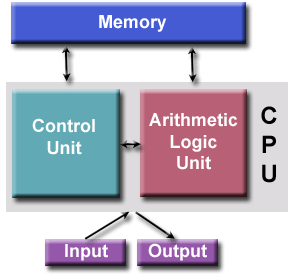
\includegraphics[width=0.7\linewidth]{figs/vonNeumann}
\caption*{Basic architecture}
\end{figure}
\end{columns}
\end{frame}


%*******************************************************************************
%******************************* Frame *****************************************
%*******************************************************************************

\begin{frame}{Serial computing}

\begin{itemize}
\item Traditionally, software has been written for serial computation:
\begin{itemize}
\item A problem is broken into a discrete series of instructions
\item Instructions are executed sequentially one after another
\item Executed on a single processor
\item Only one instruction may execute at any moment in time 
\end{itemize}

\end{itemize} 

\begin{figure}
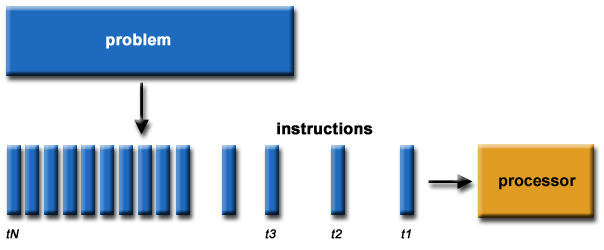
\includegraphics[width=0.7\linewidth]{figs/serial}
\caption*{}
\end{figure}
\end{frame}


%*******************************************************************************
%******************************* Frame 
%*****************************************
%*******************************************************************************

\begin{frame}{Memory model}
\begin{columns}
\column{0.49\textwidth}
\begin{figure}
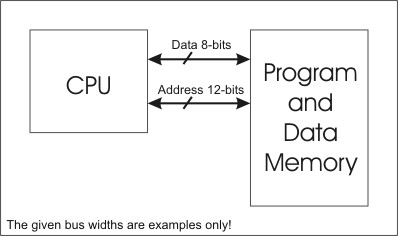
\includegraphics[width=.7\linewidth]{figs/ideal_memory_model}
\caption*{Ideal memory model: \\ We write for this architecture}
\end{figure}

\column{0.49\textwidth}
\begin{figure}
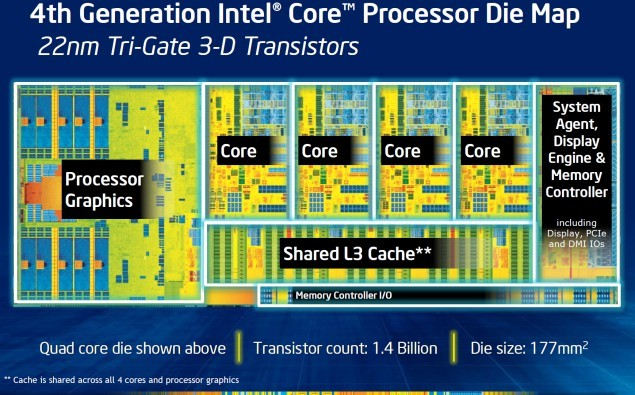
\includegraphics[width=0.9\linewidth]{figs/real_memory_model}
\caption*{Real memory model: How it actually looks}
\end{figure}
\end{columns}

\centering
\textit{The underlying assumption is cache coherency!}
\flushleft
\small
In a shared memory multiprocessor with a separate cache memory for each 
processor, it is possible to have many copies of any one instruction 
operand: one 
copy in the main memory and one in each cache memory. When one copy of an 
operand is 
changed, the other copies of the operand must be changed also. Cache 
coherency 
ensures that changes in the values of shared operands are propagated 
throughout the 
system in a timely fashion.
\end{frame}


%*******************************************************************************
%******************************* Frame 
%*****************************************
%*******************************************************************************
\begin{frame}{What are caches}
\begin{columns}
\column{0.49\textwidth}
\begin{figure}
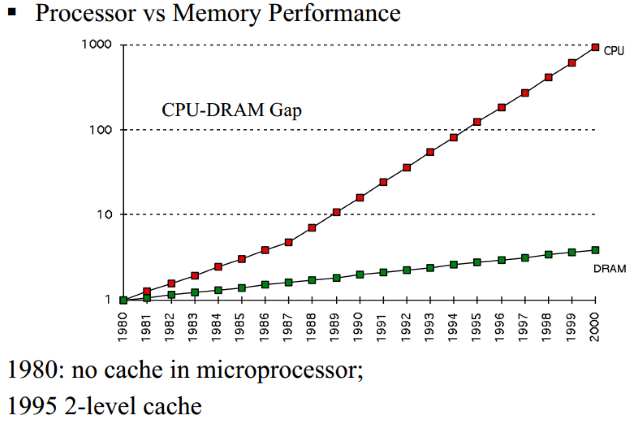
\includegraphics[width=0.9\linewidth]{figs/CPU_DRAM}
\caption*{CPU vs DRAM}
\end{figure}

\column{0.49\textwidth}
\begin{figure}
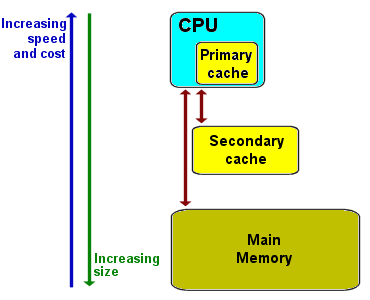
\includegraphics[width=.7\linewidth]{figs/cache}
\caption*{Cache}
\end{figure}
\end{columns}
\begin{itemize}
\item CPU caches are small pools of memory that store information the CPU 
is most 
likely to need next.

\item A cache miss means the CPU has to go scampering off to find the 
data elsewhere. This is where the L2 cache comes into play — while it's 
slower, it's 
also much larger. 

\item If data can't be found in the L2 cache, the CPU continues down the 
chain to L3 
(typically still on-die), then L4 (if it exists) and main memory (DRAM).

\end{itemize}
\end{frame}


%*******************************************************************************
%******************************* Frame *****************************************
%*******************************************************************************
\begin{frame}{Does your compiler execute the program you wrote?}

\begin{quotation}
\textbf{No, absolutely not! Compiler most often says ``you didn't intend to 
write 
that. I have a better idea...''}
\end{quotation}
\begin{itemize}
\item \textit{Sequential consistency:} Executing the program you wrote.

``the result of any execution is the same as if the operations of all the
processors were executed in some sequential order, and the operations of
each individual processor appear in this sequence in the order specified
by its program.'' - Lesslie Lamport

\item \textit{Compiler optimisation}
\item \textit{Processor execution}
\item \textit{Cache coherency}
\item Chip / compiler design annoyingly helpful:
\begin{itemize}
\item It can be expensive to exactly execute what you wrote
\item Often they rather do something else, that's faster
\end{itemize}
\end{itemize}
\end{frame}


%**************************************************************************
%******************************* Frame*************************************
%**************************************************************************
\begin{frame}[fragile]{Does your compiler execute the program you wrote?}
\begin{columns}
\column{0.5\textwidth}

\begin{minted}[mathescape, linenos,
               numbersep=5pt,
               gobble=0,
               frame=lines,
               framesep=2mm]{c++}
// Your code
for (i = 0; i < rows; ++i) {
  for (j = 0; j < cols; ++j) {
    a[j*rows+i]+=42;
  }
}
\end{minted}

\column{0.5\textwidth}
\begin{minted}[mathescape, linenos,
               numbersep=5pt,
               gobble=0,
               frame=lines, obeytabs=true, showtabs=true,
               framesep=2mm]{c++}
// Compiler optimised version
for (j = 0; j < cols; ++j) {
  for (i = 0; i < rows; ++i) {
    a[j*rows+i]+=42;
  }
}
\end{minted}
\end{columns}
\vskip3em
The CPU will expect a sequential operation. Iterating through each row of 
data is faster than going through each column. Almost always, a 2D matrix 
is stored as a 1D linear array.
\end{frame}


%**************************************************************************
%******************************* Frame*************************************
%**************************************************************************
\begin{frame}{Stack v Heap}
\begin{columns}
\column{0.65\textwidth}
\begin{itemize}
\item \textit{Stack:} Stores local data, return
addresses, used for parameter
passing. e.g., int i; 
\item typically stored in the ``low'' addresses of memory and 
fills upward toward its upper limit. 

\item faster, but smaller in size. Last In Fist Out.

\item \textit{Heap:} You would use the heap if you don't know exactly how much
data you will need at runtime or if you need to allocate a lot of data.

$ClassObj* obj = new ClassObj\{0\};  ... delete\mathrm{ obj};$

$auto obj = std::make\_shared < ClassObj>(0);$

\item Stored at the ``top'' of the address space and grows 
towards the stack. 

\item Slower but larger in size

\item Use local variables (stack) when you can. Use dynamic
allocation (heap) when you have to.

\end{itemize}

\column{0.35\textwidth}
\begin{figure}
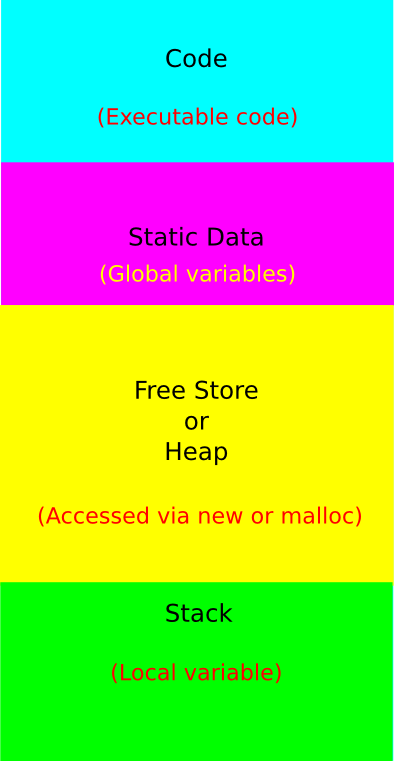
\includegraphics[width=.8\linewidth]{figs/stack_heap}
\caption*{Stack v Heap}
\end{figure}

\end{columns}
\end{frame}

%*******************************************************************************
%******************************* Frame *****************************************
%*******************************************************************************
\section{Parallel computing}

\begin{frame}{What is parallel computing?}
%\begin{columns}
%\column{.6\linewidth}
In the simplest sense, parallel computing is the simultaneous use of multiple 
compute resources to solve a computational problem:
\begin{itemize}
\item A problem is broken into discrete parts that can be solved concurrently
\item Each part is further broken down to a series of instructions
\item Instructions from each part execute simultaneously on different processors
\item An overall control/coordination mechanism is employed 
\end{itemize}
%\column{.495\linewidth}
\begin{figure}
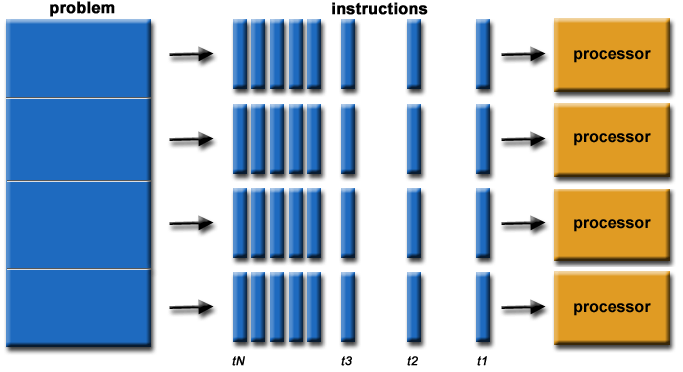
\includegraphics[width=0.7\linewidth]{figs/parallel_problem.png}
\caption*{}
\end{figure}
%\end{columns}
\end{frame}

%*******************************************************************************
%******************************* Frame *****************************************
%*******************************************************************************
\begin{frame}{Concurrency v Parallelism}
\begin{columns}
\column{0.49\linewidth}
\begin{figure}
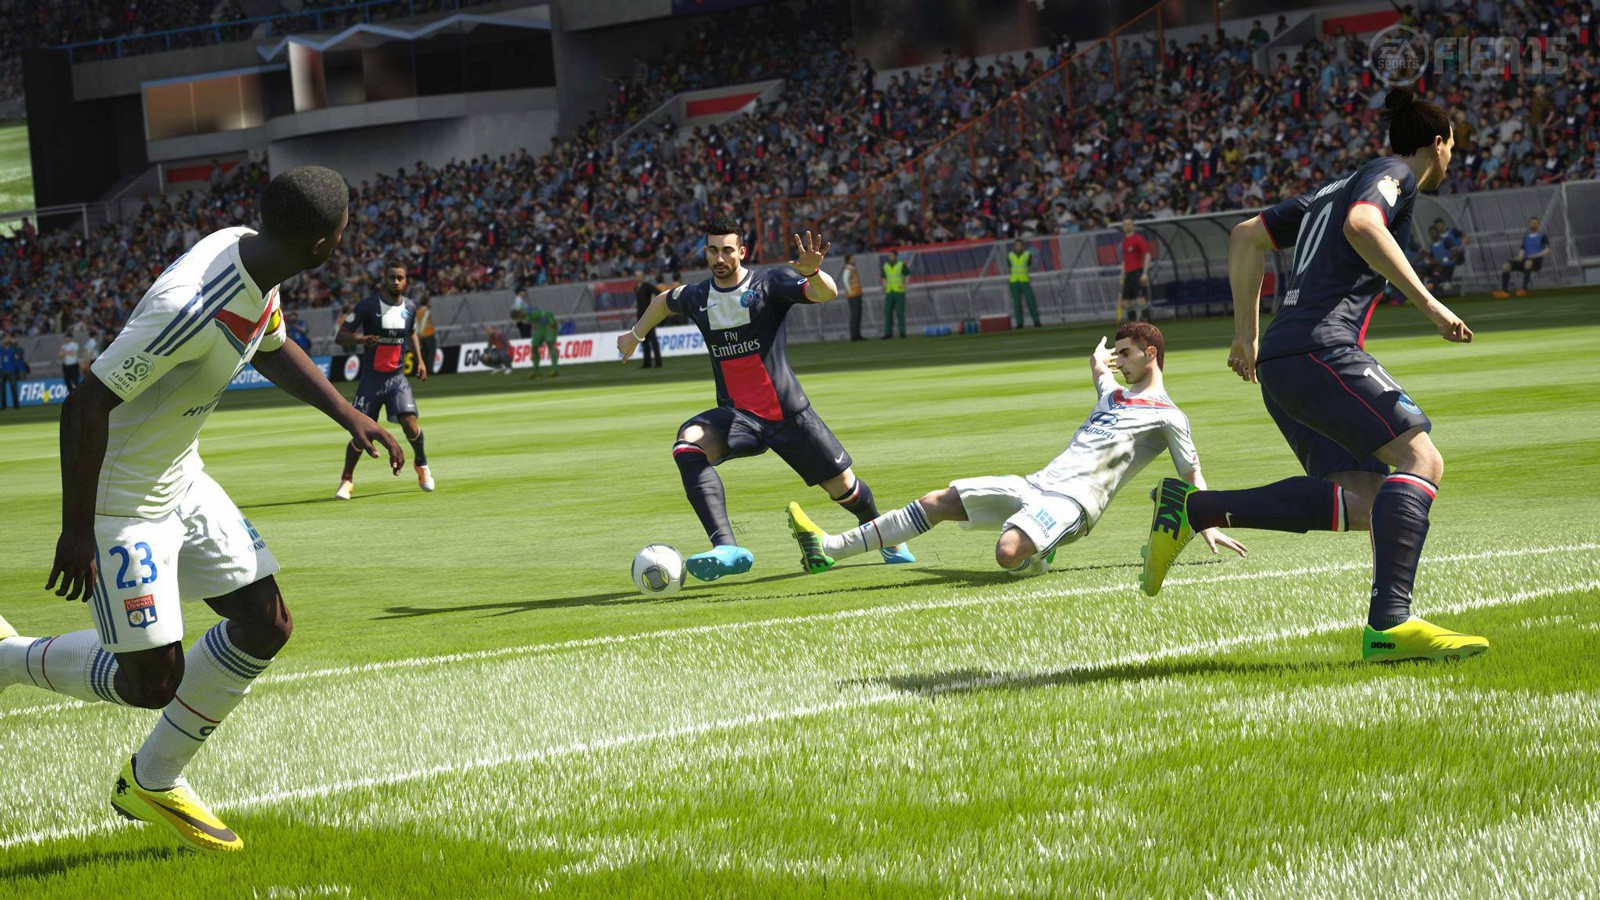
\includegraphics[width=\linewidth]{figs/concurrency.png}
\caption*{Concurrency}
\end{figure}
\column{0.49\linewidth}
\begin{figure}
\includegraphics[width=\linewidth]{figs/parallelism.png}
\caption*{parallelism}
\end{figure}
\end{columns}
\end{frame}


%*******************************************************************************
%******************************* Frame *****************************************
%*******************************************************************************
\begin{frame}{Flynn's Classical Taxonomy}

\begin{figure}
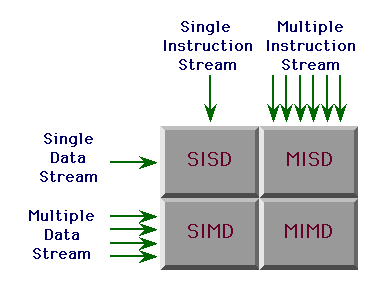
\includegraphics[width=0.7\linewidth]{figs/flynn}
\caption*{Computer architecture}
\end{figure}
\end{frame}

%*******************************************************************************
%******************************* Frame *****************************************
%*******************************************************************************
\begin{frame}{Cost of parallelisation}
\begin{columns}

\column{0.49\linewidth}
$speedup = \frac{1}{1 - \mathrm{parallel part}}$
\begin{figure}
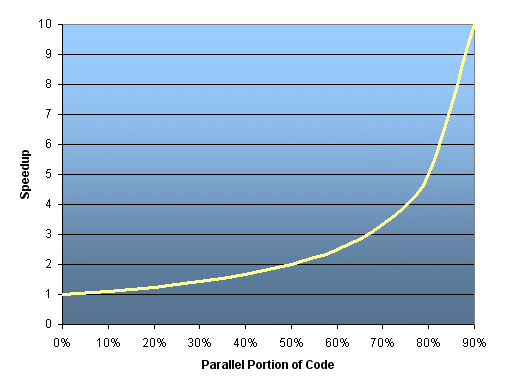
\includegraphics[width=\linewidth]{figs/amdahl1}
\caption*{Single processor}
\end{figure}
\column{0.49\linewidth}
$speedup = \frac{1}{\frac{\mathrm{parallel part}}{\mathrm{\# processors}} + 
\mathrm{serial part}}$
\begin{figure}
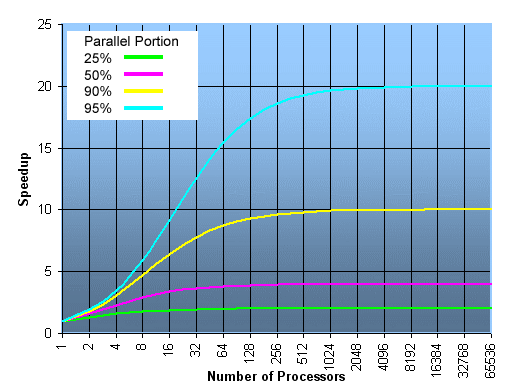
\includegraphics[width=\linewidth]{figs/amdahl2}
\caption*{Multiple processor}
\end{figure}
\end{columns}

Problems that increase the percentage of parallel time with their size are more 
\textbf{\textit{scalable}} than problems with a fixed percentage of parallel time

\end{frame}


%*******************************************************************************
%******************************* Frame *****************************************
%*******************************************************************************
\begin{frame}{Scalability}
\begin{itemize}
\item \textit{Strong scaling:} The total problem size stays fixed as more processors 
are added. 
\item \textit{Weak scaling:} The problem size per processor stays fixed as more 
processors are added. 

\item Simply adding more processors is rarely the answer to scalability.

\item The algorithm may have inherent limits to scalability. At some point, adding 
more resources causes performance to decrease. 

\item Hardware factors play a significant role in scalability. Examples:

\begin{itemize}
\item Memory-cpu bus bandwidth on Symmetric Multi-Processor (SMP) -
    where multiple processors share a single 
    address space and have equal access to all resources. 
\item Communications network bandwidth
\item Amount of memory available on any given machine or set of machines
\item Processor clock speed 
\end{itemize}

\item Parallel support libraries and subsystems software can limit scalability 
independent of your application. 
\end{itemize}
\end{frame}

%*******************************************************************************
%******************************* Frame *****************************************
%*******************************************************************************
\section{Shared memory}
\begin{frame}{Shared memory}
\begin{itemize}
\item Multiple processors can operate independently but share the same memory 
resources.

\item Changes in a memory location effected by one processor are visible to all 
other processors. 

\item Data sharing between tasks is both fast and uniform due to the proximity of 
memory to CPUs 

\item Primary disadvantage is the lack of scalability between memory and CPUs
\end{itemize}

\begin{columns}
\column{0.49\linewidth}
\begin{figure}
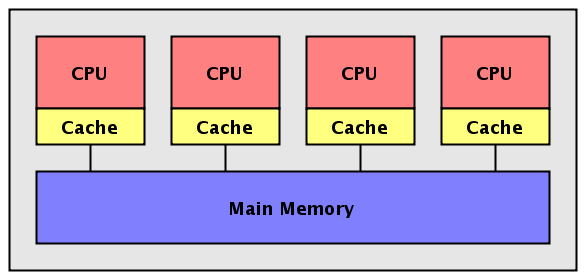
\includegraphics[width=0.7\linewidth]{figs/shared_memory.png}
\caption*{Shared memory}
\end{figure}
\column{0.49\linewidth}
\begin{figure}
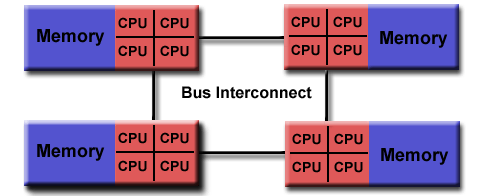
\includegraphics[width=0.7\linewidth]{figs/numa.png}
\caption*{Non Uniform Memory access}
\end{figure}
\end{columns}
\begin{columns}
\column{0.6\linewidth}
If we want thread 0 to use the value placed in the array by thread 1, we needs to 
use a mechanism which assures that thread 1 has written the value before thread 0 
reads it.
\column{0.35\linewidth}
\begin{figure}
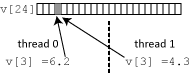
\includegraphics[width=\linewidth]{figs/shared_memory_vector.png}
\end{figure}
\end{columns}
\end{frame}


%*******************************************************************************
%******************************* Frame *****************************************
%*******************************************************************************
\begin{frame}{Shared memory frameworks}
\begin{itemize}
\item \textbf{OpenMP}
\begin{itemize}
\item API that supports multi-platform shared memory multiprocessing programming
\item Model: master thread forks 
\item Simple to use
\end{itemize}

\item \textbf{POSIX threads or p-threads}
\begin{itemize}
\item Library based set of C language types, functions and constants. 
\item A thread can be created with much less operating system overhead.
\item No advanced threading algorithm. Use C++11 with same set of features.
\end{itemize}

\item \textbf{C++11 threads}
\begin{itemize}
\item C++11 language provides a memory model that supports threading.
\item This library provides everything from thread management to mutexes and 
synchronization. 
\end{itemize}

\item \textbf{Intel Cilk}
\begin{itemize}
\item Language extension.
\item Simple to parallelise.
\item No advanced algorithm support.
\end{itemize}

\item \textbf{Intel Threaded Building Blocks}
\begin{itemize}
\item C++ template library for parallelisation.
\item Support for parallel algorithms, data structures and is scalable.
\end{itemize}
\end{itemize}

\end{frame}


%*******************************************************************************
%******************************* Frame *****************************************
%*******************************************************************************
\begin{frame}{Shared memory: Choosing the right framework}

\begin{figure}
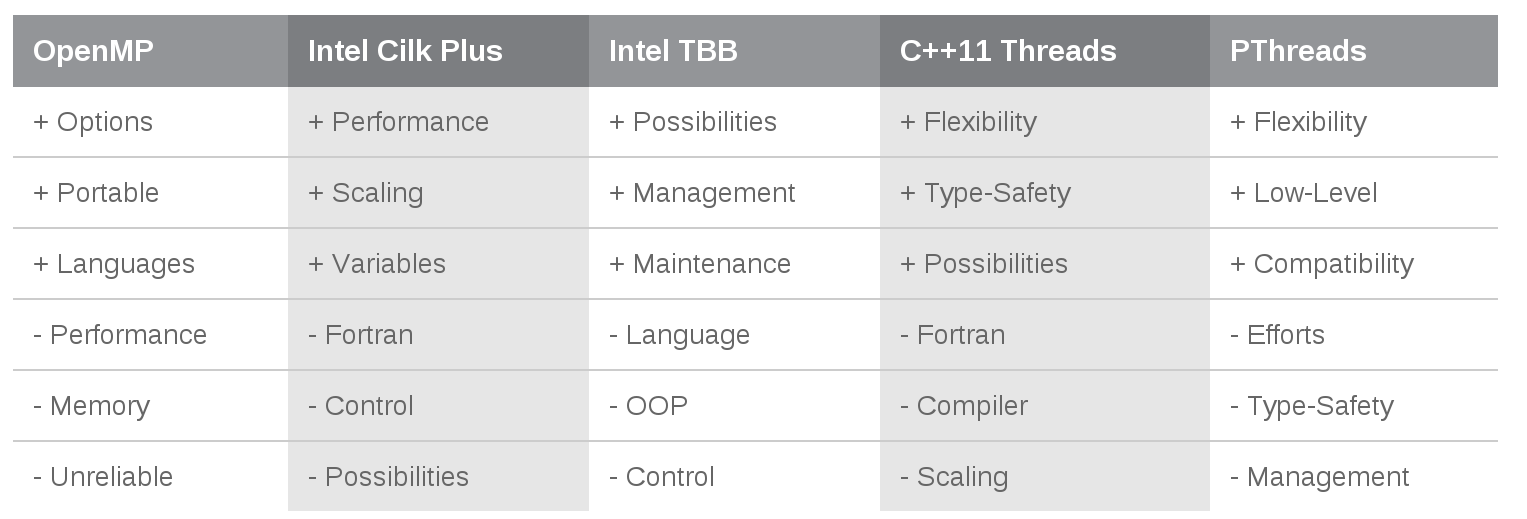
\includegraphics[width=\linewidth]{figs/shared_memory_comparison.png}
\end{figure}
\end{frame}

%*******************************************************************************
%******************************* Frame *****************************************
%*******************************************************************************
\begin{frame}{OpenMP}
\begin{itemize}
\item Open Multi-Processing is an API to explicitly direct multi-
threaded, shared memory parallelism
\item Comprised of three primary API components:
\begin{itemize}
\item Compiler Directives – Pragmas (pre-processor macros)
\item Runtime Library Routines
\item Environment Variables
\end{itemize}
\item The programmer is responsible for synchronizing input and
output.
\item OpenMP uses threads. A thread of execution is the smallest unit of processing 
that can be scheduled by an operating system.
\item Threads exist within the resources of a single process. Without
the process, they cease to exist.
\item Typically, the number of threads match the number of machine
processors/cores. However, the actual use of threads is up to the
application.
\end{itemize}
\end{frame}

%*******************************************************************************
%******************************* Frame *****************************************
%*******************************************************************************
\begin{frame}{Fork – Join Model}

\begin{figure}
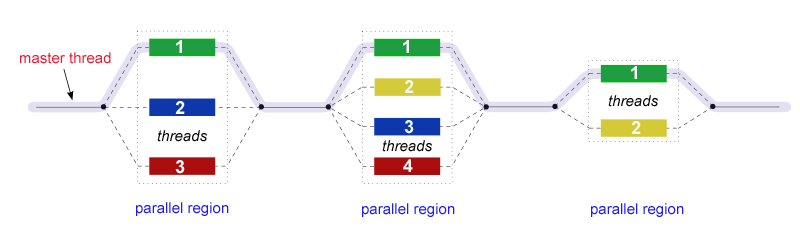
\includegraphics[width=\linewidth]{figs/fork_join}
\caption*{Fork - Join model}
\end{figure}

\begin{itemize}
\item \textbf{FORK}: the master thread then creates a team of parallel threads.
The statements in the program that are enclosed by the parallel region
construct are then executed in parallel among the various team
threads.
\item \textbf{JOIN}: When the team threads complete the statements in the parallel
region construct, they synchronize and terminate, leaving only the
master thread.
\item The number of parallel regions and the threads that comprise them are
arbitrary.
\end{itemize}
\end{frame}
%*******************************************************************************
%******************************* Frame *****************************************
%*******************************************************************************
\begin{frame}[fragile]{OpenMP: Code structure}

\begin{minted}[mathescape, linenos,
               numbersep=5pt,
               gobble=0,
               frame=lines,
               framesep=2mm]{c++}
#include <omp.h>
int main () {
  int var1, var2, var3;
  // Serial code . . .
  // Beginning of parallel section. Fork a team of threads.
  //Specify variable scoping
#pragma omp parallel for private(var1, var2) shared(var3) {
    // Parallel section executed by all threads
    // Run-time Library calls
    // All threads join master thread and disband
  }
  // Resume serial code ..
}
\end{minted}
\end{frame}

%*******************************************************************************
%******************************* Frame *****************************************
%*******************************************************************************
\begin{frame}[fragile]{OpenMP: Dot product}
Dot product $sum += a[N] * b[N]$
\begin{columns}
\column{0.45\linewidth}
\begin{minted}[mathescape, linenos,
               numbersep=5pt,
               gobble=0,
               frame=lines,
               framesep=2mm]{c++}
// serial code
const int size = 100;
int main() {
  int i;
  float a[size], b[size];
  float sum = 0.0;
  // Some initializations
  for (i = 0; i < size; i++) 
    a[i] = b[i] = 1.0;
  // computation loop
  for (i = 0; i < size; i++) 
    sum += (a[i] * b[i]);

  printf("Sum = %f\n", sum);
}
\end{minted}
\column{0.45\linewidth}
\begin{minted}[mathescape, linenos,
               numbersep=5pt,
               gobble=0,
               frame=lines,
               framesep=2mm]{c++}
// parallel code
const int size = 100;
int main() {
  int i;  float sum = 0.0;
  float a[size], b[size];

  for (i = 0; i < size; i++) 
    a[i] = b[i] = 1.0;

#pragma omp parallel for \
default(shared) private(i) 
  for (i = 0; i < size; i++) 
    sum += (a[i] * b[i]);

  printf("Sum = %f\n", sum);
}  
\end{minted}
\end{columns}
\end{frame}


%*******************************************************************************
%******************************* Frame *****************************************
%*******************************************************************************
\begin{frame}[fragile]{Parallel dot product: What went wrong?}
\begin{columns}
\column{0.47\linewidth}
\begin{minted}[mathescape, linenos,
               numbersep=5pt,
               gobble=0,
               frame=lines,
               framesep=2mm]{c++}
// wrong code
const int size = 100;
int main() {
  int i;  float sum = 0.0;
  float a[size], b[size];
  for (i = 0; i < size; i++) 
    a[i] = b[i] = 1.0;

#pragma omp parallel for \
default(shared) private(i) 
  for (i = 0; i < size; i++) 
    sum += (a[i] * b[i]);

  printf("Sum = %f\n", sum);
}  
\end{minted}
\column{0.49\linewidth}
\begin{minted}[mathescape, linenos,
               numbersep=5pt,
               gobble=0,
               frame=lines,
               framesep=2mm]{c++}
// parallel code
const int size = 100;
int main() {
  int i;  float sum = 0.0;
  float a[size], b[size];
  for (i = 0; i < size; i++) 
    a[i] = b[i] = 1.0;

#pragma omp parallel for \
default(shared) private(i) \
    reduction(+ : sum)
  for (i = 0; i < size; i++) 
    sum += (a[i] * b[i]);

  printf("Sum = %f\n", sum);
}  
\end{minted}
\end{columns}

Synchronisation! Don't forget to synchronise the threads
\end{frame}




%*******************************************************************************
%******************************* Frame *****************************************
%*******************************************************************************
\begin{frame}[fragile]{Auto vectorization}
\begin{itemize}
\item A special case of automatic parallelisation, where a computer program is 
converted from a scalar implementation, which processes a single pair of operands at 
a time, to a vector implementation, which processes one operation on multiple pairs 
of operands at once.
\item The Auto-Vectorizer analyzes loops in your code, and uses the
vector registers and instructions on the target computer to execute
them, if it can. This can improve the performance of your code.
\end{itemize}
\begin{columns}
\column{0.47\linewidth}
\begin{minted}[mathescape, linenos,
               numbersep=5pt,
               gobble=0,
               frame=lines,
               framesep=2mm]{c++}
// sequential code

for (int i = 0; i < 1000; ++i) {
  //32-bit operation
  A[i] = B[i]*C[i]; 
}
\end{minted}
\column{0.49\linewidth}
\begin{minted}[mathescape, linenos,
               numbersep=5pt,
               gobble=0,
               frame=lines,
               framesep=2mm]{c++}
// vectorized code
for (int i = 0; i < 1000; i+=4) {
  A[i:i+3] = mulps(B[i:i+3]*C[i:i+3]);
  // 128-bit operation
  // Which is 4x32bit operations
  // Takes the same amount of time  
}
\end{minted}
\end{columns}

\end{frame}

%*******************************************************************************
%******************************* Frame *****************************************
%*******************************************************************************
\begin{frame}{Auto vectorization: How it works}
\begin{figure}
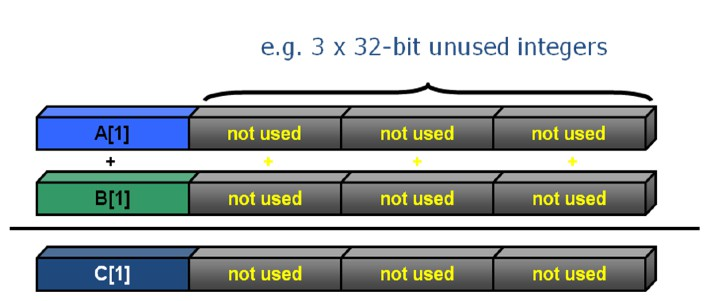
\includegraphics[width=.7\linewidth]{figs/novectorization.png}
\caption*{No vectorization}
\end{figure}
\begin{figure}
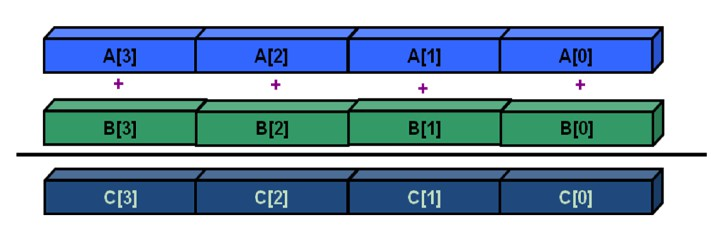
\includegraphics[width=.7\linewidth]{figs/vectorized.png}
\caption*{Vectorized version}
\end{figure}

\end{frame}

%*******************************************************************************
%******************************* Frame *****************************************
%*******************************************************************************
\begin{frame}{SIMD parallelisation in loops}
\begin{itemize}
\item Loop level parallelism
\begin{itemize}
\item SIMD for a single statement across consecutive iterations
\item Handles misaligned data
\item Patterns such as reduction, linear recursion
\end{itemize}
\item SIMD across entire loop iterations
\item Effectively collapse innermost loop
\end{itemize}
\begin{figure}
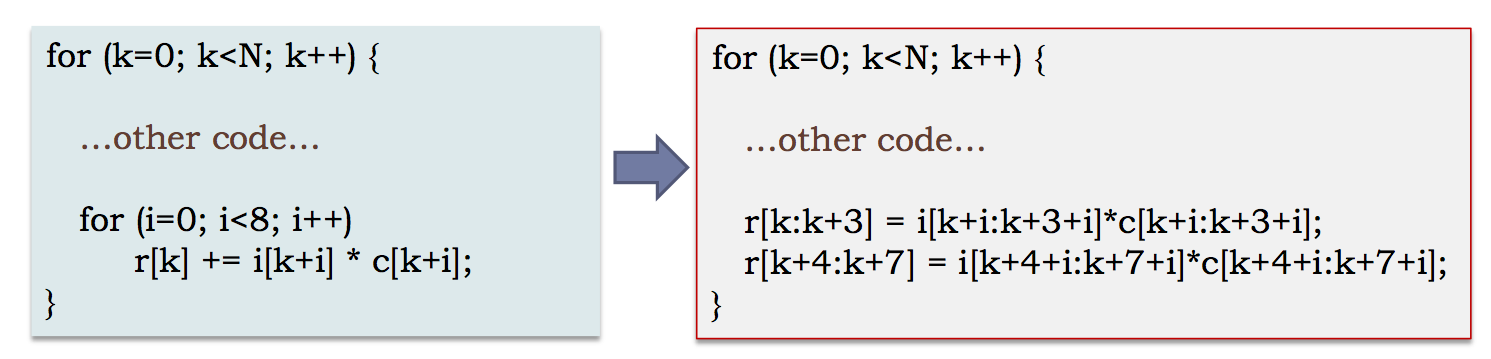
\includegraphics[width=\linewidth]{figs/simd_loop.png}
\caption*{SIMD nested loops}
\end{figure}
\end{frame}

%*******************************************************************************
%******************************* Frame *****************************************
%*******************************************************************************
\begin{frame}{SIMD parallelisation in loops}
\begin{figure}
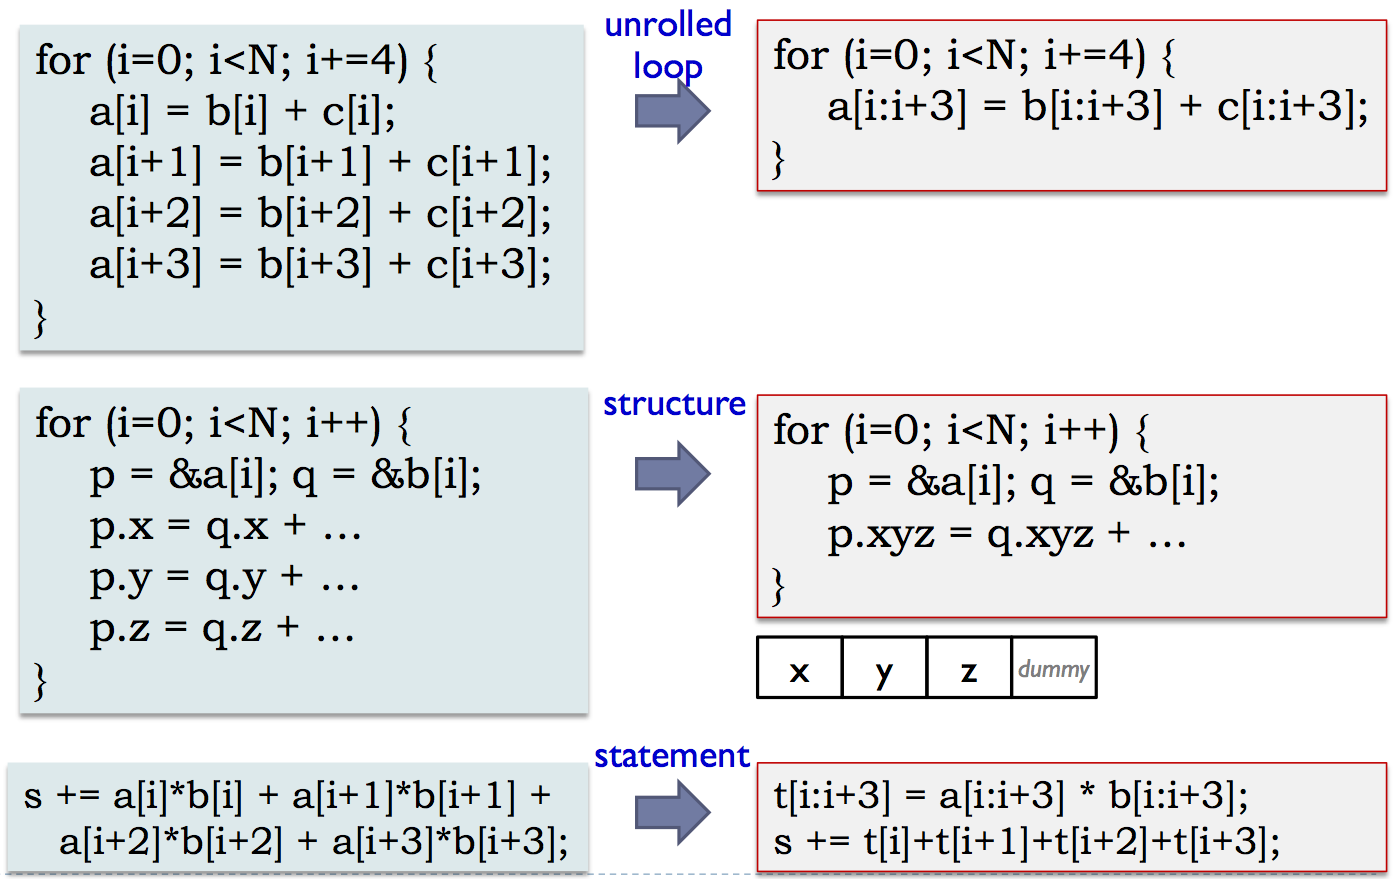
\includegraphics[width=\linewidth]{figs/simd_parallelisation.png}
\end{figure}
\end{frame}



%*******************************************************************************
%******************************* Frame *****************************************
%*******************************************************************************
\section{Distributed memory}
\begin{frame}{Distributed memory}
\begin{itemize}
\item \textbf{General Characteristics:}
\begin{itemize}
\item Distributed memory systems require a communication network to 
connect inter-processor memory. Usually via Ethernet.

\item Processors have their own local memory. Memory addresses in one processor do 
not map to another processor, so there is no concept of global address space across 
all processors.

\item Because each processor has its own local memory, it operates independently. 
Changes it makes to its local memory have no effect on the memory of other     
processors. Hence, the concept of cache coherency does not apply.

\item When a processor needs access to data in another processor, it is usually the 
task of the programmer to explicitly define how and when data is communicated.

\end{itemize}

\end{itemize}
\begin{figure}
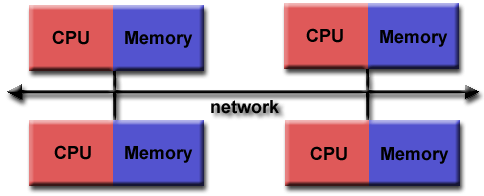
\includegraphics[width=0.5\linewidth]{figs/distributed_memory}
\end{figure}
\end{frame}


%*******************************************************************************
%******************************* Frame *****************************************
%*******************************************************************************
\begin{frame}{Distributed memory: Advantages and disadvantages}
\begin{itemize}

\item \textbf{Advantages:}
\begin{itemize}
\item Memory is scalable with the number of processors. 
\item Increase the number of processors and the size of memory increases 
proportionately.
\item Each processor can rapidly access its own memory without interference and 
    without the overhead incurred with trying to maintain global cache coherency.
\item Cost effectiveness: can use commodity, off-the-shelf processors and 
networking. 
\end{itemize}
\item \textbf{Disadvantages:}
\begin{itemize}
\item The programmer is responsible for many of the details associated with data 
    communication between processors.
\item It may be difficult to map existing data structures, based on global memory, 
to this memory organization.
\item Non-uniform memory access times - data residing on a remote node takes longer 
to access than node local data. 

\end{itemize}
\end{itemize}
\end{frame}


%*******************************************************************************
%******************************* Frame *****************************************
%*******************************************************************************
\begin{frame}{MPI: Message Passing Interface}
\begin{columns}
\column{0.6\linewidth}
\begin{itemize}
\item OpenMPI, MPICH, IntelMPI, BoostMPI
\item MPI libraries vary in their level of thread support:
\begin{itemize}
\item $MPI\_THREAD\_SINGLE$ - Level 0: Only one thread will execute.

\item $MPI\_THREAD\_FUNNELED$ - Level 1: The process may be multi-threaded, but 
only the main thread will make MPI calls - all MPI calls are funneled to the main 
thread.

\item $MPI\_THREAD\_SERIALIZED$ - Level 2: The process may be multi-threaded, and 
multiple threads may make MPI calls, but only one at a time. That is, calls are not 
made concurrently from two distinct threads as all MPI calls are serialized.

\item $MPI\_THREAD\_MULTIPLE$ - Level 3: Multiple threads may call MPI with no 
    restrictions. 
\end{itemize}
\end{itemize}
\column{0.4\linewidth}
\begin{figure}
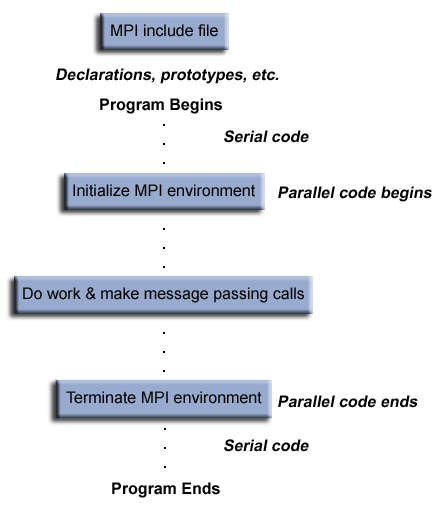
\includegraphics[width=\linewidth]{figs/mpi.png}
%\caption*{SIMD nested loops}
\end{figure}
\end{columns}
\end{frame}

%*******************************************************************************
%******************************* Frame *****************************************
%*******************************************************************************
\begin{frame}{Domain decomposition}
\begin{itemize}
\item Tasks are statically or semi-statically mapped onto processes based on spatial 
location; each task performs similar operations on different data (subdomains).
\item Work is interspersed with communication to synchronize the tasks or share data.
\item The degree of parallelism increases with problem size, enabling effective use 
of more processes on larger problems.
\end{itemize}
\begin{columns}
\column{0.4\linewidth}
\begin{figure}
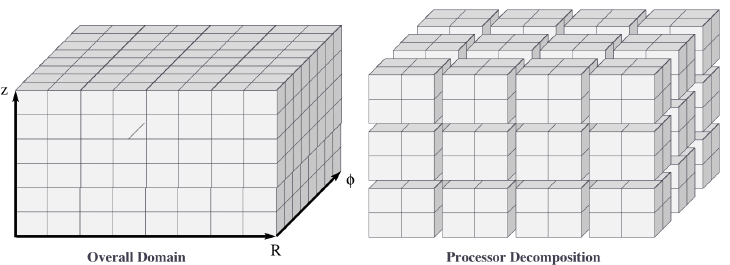
\includegraphics[width=\linewidth]{figs/decomp_3D.png}
\caption*{Domain decomposition}
\end{figure}
\column{0.6\linewidth}
\begin{figure}
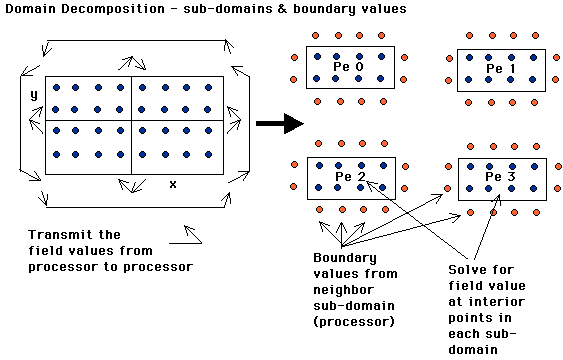
\includegraphics[width=\linewidth]{figs/domain_decomposition.png}
%\caption*{Domain decomposition communication}
\end{figure}

\end{columns}
\end{frame}


%*******************************************************************************
%******************************* Frame *****************************************
%*******************************************************************************
\begin{frame}{Hybrid Distributed-Shared Memory}
\begin{itemize}
\item Largest and fastest computers employ hybrid architectures.
\item The shared memory component can be a shared memory machine and/or graphics 
    processing units (GPU).

\item The distributed memory component is the networking of multiple shared 
memory/GPU machines, which know only about their own memory - not the memory on 
another machine. Therefore, network communications are required to move data from 
one machine to another.

\item \textbf{Advantages and Disadvantages:}

\begin{itemize}
\item shared and distributed memory architectures.
\item Increased scalability is an important advantage
\item Increased programmer complexity
\end{itemize}
\end{itemize}
\begin{columns}
\column{0.45\linewidth}
\begin{figure}
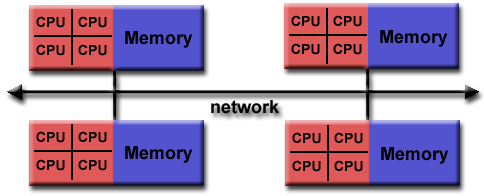
\includegraphics[width=\linewidth]{figs/hybrid_mem.png}
%\caption*{SIMD nested loops}
\end{figure}
\column{0.45\linewidth}
\begin{figure}
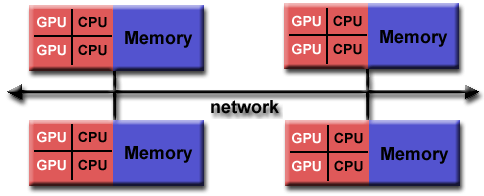
\includegraphics[width=\linewidth]{figs/hybrid_gpu.png}
%\caption*{SIMD nested loops}
\end{figure}
\end{columns}
\end{frame}

%*******************************************************************************
%******************************* Frame *****************************************
%*******************************************************************************
\section{Graphics Processing Units}
\begin{frame}{Trends in HPC}
\begin{columns}
\column{0.4\linewidth}
\begin{figure}
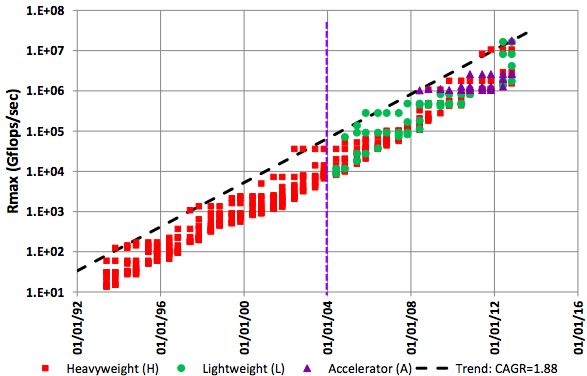
\includegraphics[width=\linewidth]{figs/flops.png}
\caption*{FLOPS}
\end{figure}
\column{0.4\linewidth}
\begin{figure}
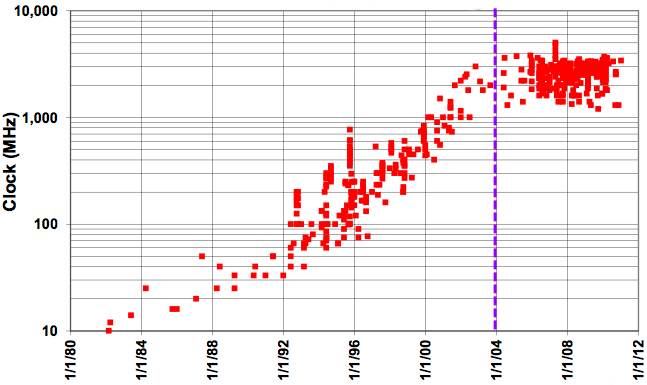
\includegraphics[width=\linewidth]{figs/clocks.png}
\caption*{Clock speed}
\end{figure}
\end{columns}
\begin{columns}
\column{0.4\linewidth}
\begin{figure}
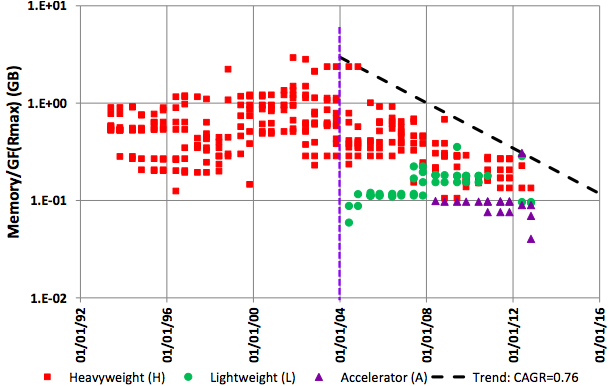
\includegraphics[width=\linewidth]{figs/memory_flops.png}
\caption*{Memory / flop}
\end{figure}
\column{0.4\linewidth}
More Flop/s per clock cycle and less memory per Flop/s means Flop/s
are ``free'' but there is a price: complexity in programmability!

\end{columns}
\end{frame}


%*******************************************************************************
%******************************* Frame *****************************************
%*******************************************************************************
\begin{frame}{Graphics Processing Units (GPU)}
\begin{columns}
\column{0.49\linewidth}
\begin{figure}
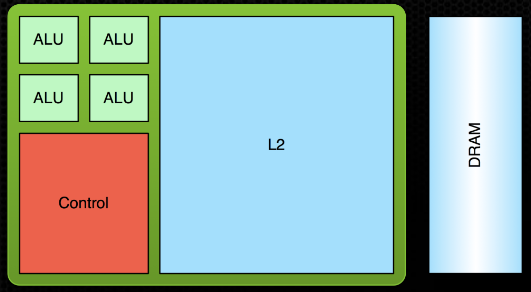
\includegraphics[width=\linewidth]{figs/CPU.png}
\caption*{CPU}
\end{figure}
\begin{itemize}
\item Optimized for low-latency access to cached data sets
\item Control logic for out-of-order and speculative execution
\item 10’s of threads
\end{itemize}

\column{0.49\linewidth}
\begin{figure}
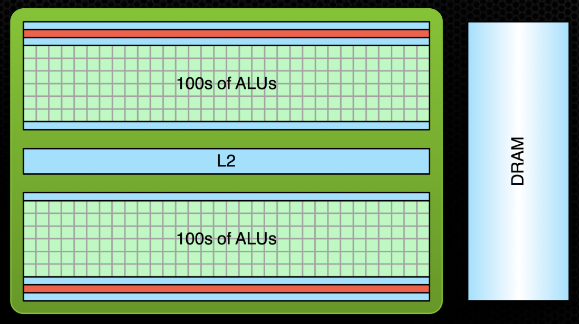
\includegraphics[width=\linewidth]{figs/GPU.png}
\caption*{GPU}
\end{figure}
\begin{itemize}
\item Optimized for data-parallel, throughput computation
\item Architecture tolerant of memory latency
\item More transistors dedicated to computation
\item 10000’s of threads
\end{itemize}


\end{columns}
\end{frame}

%*******************************************************************************
%******************************* Frame *****************************************
%*******************************************************************************
\begin{frame}{Low Latency or High Throughput?}
\begin{itemize}
\item CPU architecture must minimize latency within each thread
\item GPU architecture hides latency with computation from other thread warps
\end{itemize}
\begin{figure}
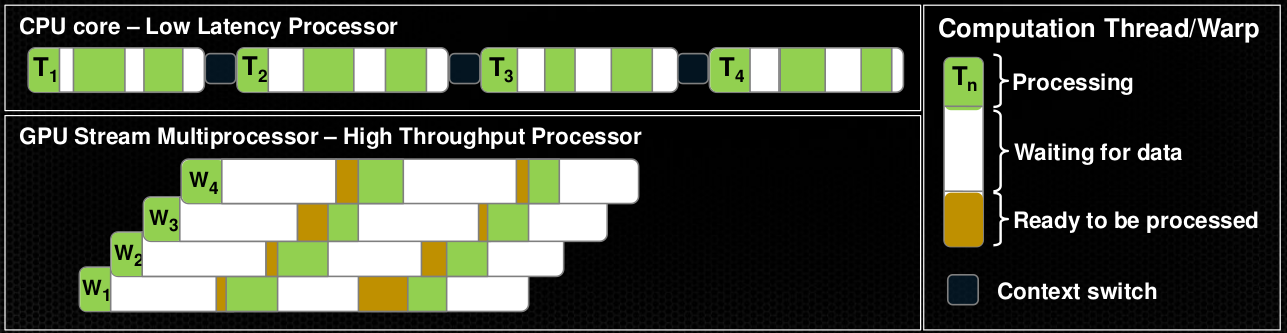
\includegraphics[width=\linewidth]{figs/CPU_GPU_Latency.png}
\caption*{GPU}
\end{figure}
\end{frame}


%*******************************************************************************
%******************************* Frame *****************************************
%*******************************************************************************
\begin{frame}{CPU v GPU}
\begin{columns}
\column{0.49\linewidth}
\begin{figure}
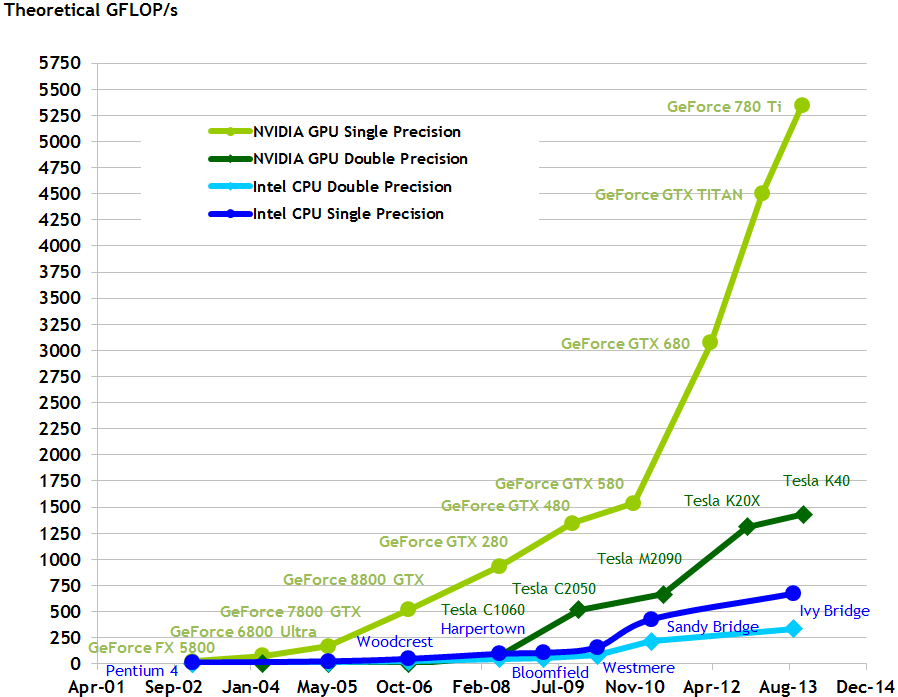
\includegraphics[width=\linewidth]{figs/CPU_GPU_FLOPS.png}
\caption*{FLOPS}
\end{figure}
\column{0.49\linewidth}
\begin{figure}
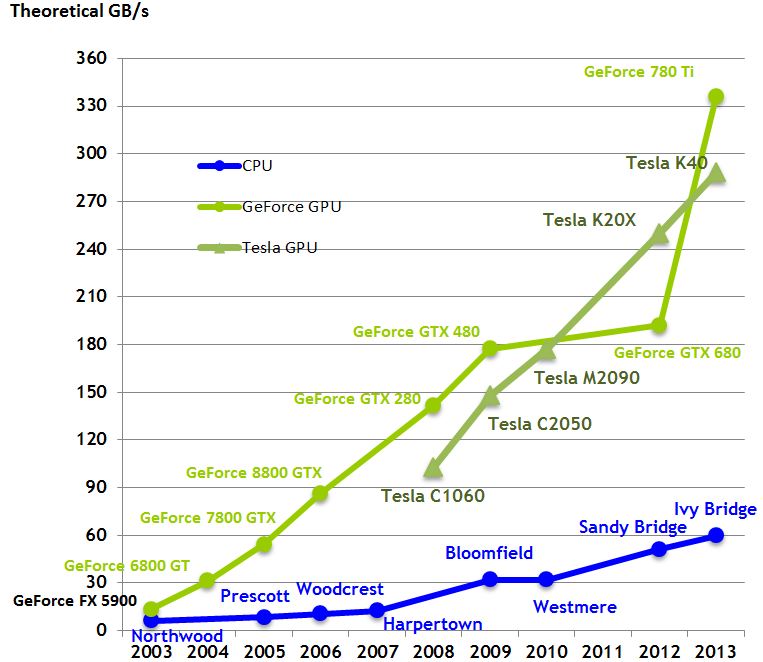
\includegraphics[width=\linewidth]{figs/CPU_GPU_Bandwidth.png}
\caption*{Bandwidth}
\end{figure}
\end{columns}
\end{frame}

%*******************************************************************************
%******************************* Frame *****************************************
%*******************************************************************************
\begin{frame}{NVIDIA K20 GPU architecture}
\begin{columns}
\column{0.49\linewidth}
\begin{itemize}
\item SMX = Streaming multi processor
\begin{itemize}
\item 192 cores
\item 64k registers
\item 64KB of shared memory and L1 cache
\item 8KB cache for constants
\item up to 2K active threads
\end{itemize}
\item Each K20 has 13 SMX...
\begin{itemize}
\item 200 GB/s
\item 1.1 TFlops (peak)
\item 225 Watt (peak)
\end{itemize}
\end{itemize}
\column{0.49\linewidth}
\begin{figure}
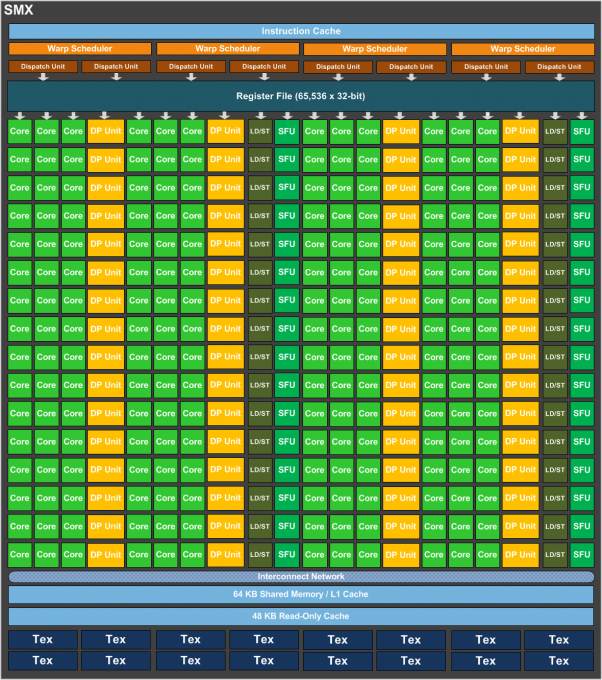
\includegraphics[width=\linewidth]{figs/GPU_layout.png}
\caption*{Bandwidth}
\end{figure}
\end{columns}
\end{frame}

%*******************************************************************************
%******************************* Frame *****************************************
%*******************************************************************************
\begin{frame}{GPU workflow}
\begin{columns}
\column{0.49\linewidth}

\begin{itemize}
\item The HOST (CPU) copies data to the DEVICE (GPU) memory
\item The HOST triggers the DEVICE execution
\item The DEVICE executes instructions asynchronously
\item The HOST retrieves the results from the DEVICE memory
\end{itemize}
\column{0.49\linewidth}
\begin{figure}
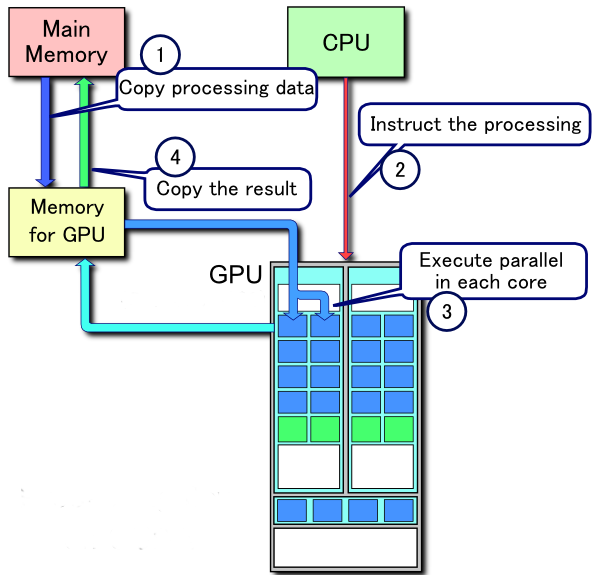
\includegraphics[width=\linewidth]{figs/GPU_Workflow.png}
%\caption*{GPU }
\end{figure}
\end{columns}
\end{frame}

\end{document}